\section{Theorie}

\subsection{organische Szintillatoren}

Szintillatoren sind  Materialien die bei Bestrahlung mit energiereichen Photonen oder geladenen Teilchen angeregt werden und die Anregungsenergie in Form von Licht wieder abgeben. Organische Szintillatoren bestehen wie der Name schon vermuten lässt vorwiegend aus Kohlenstoff, Wasserstoff, Sauerstoff und Stickstoff wie es auch in z.B. menschlichem Gewebe der Fall ist. Es liegt daher nahe Detektoren auf Basis organischer Szintillatoren für die Dosismessung im Strahlenschutz zu verwenden. Organische Szintillatoren bestehen typischerweise aus zwei Komponenten: Einem primären Fluoreszenzstoff (z.B. auf Basis von Polyvinyltoluol) und einem \glqq Wellenlängenschieber \grqq{} (z.B. POPOP) da die vom primären Fluoreszenzstoff abgegebenen UV-Strahlen in den meisten durchsichtigen Materialien eine nur sehr geringe Reichweite besitzen.

\subsection{Wechselwirkung von Photonen mit Materie}

Obwohl Photonen in vieler Weise mit Materie wechselwirken können sind für diesen Versuch nur zwei Prozesse von wesentlicher Bedeutung: Die Compton-Streuung und der Photoeffekt. In den folgenden Abschnitten werden beide näher erläutert.

\subsubsection{Photoeffekt}

Der Photoeffekt beschreibt die Anregung von Elektronen durch Absorption eines Photons.
Für den HPGe-Detektor ist vor allem der innere photoelektrische Effekt von Bedeutung. Er beschreibt die Zunahme der Leitfähigkeit eines Halbleiters durch Bildung von nicht aneinander gebundenen Elektron-Loch-Paaren. Der HPGe-Detektor besteht aus einem hochreinen Germanium-Kristall der zwischen einem $n^{+}$ Kontakt (typ. durch Lithium-eindiffusion) am positiven Spannungspol und einem $p^{+}$ Kontakt (typ. durch Bor-implantation) am negativen Spannungspol sitzt; Der Detektor insgesamt entspricht einer Halbleiterdiode in Sperrichtung. Trifft ein Photon auf den Detektor und erzeugt ein Elektron-Loch-Paar werden durch die anliegende Spannung Elektron und Loch abgesaugt und bilden so einen detektierbaren Verschiebungsstrom. Dafür muss das einfallende Photon natürlich genügend Energie besitzen um die Bandlücke zu überwinden (Für Germanium \SI{0.67}{\electronvolt}), praktisch jedoch deutlich mehr um das Siganl-Rausch-Verhältnis groß genug zu bekommen. So werden bei einfallenden Photonen von \SI{1}{\mega\electronvolt} etwa \num{3e5} Elektron-Loch-Paare erzeugt \cite{HPGe-Detektor}. Da bei Raumtemperatur eine ständige thermische Anregung der Elektronen enormes Signalrauschen verursachen würde ist eine Abkühlung mit flüssigem Stickstoff notwendig.
Für den zu kalibrierenden Detektor ist vor allem der äußere photoelektrische Effekt von Bedeutung, genauer für den Photoelektronenvervielfacher (Abb. \ref{theorie_PEV}).

\begin{figure}[ht]
	\centering
    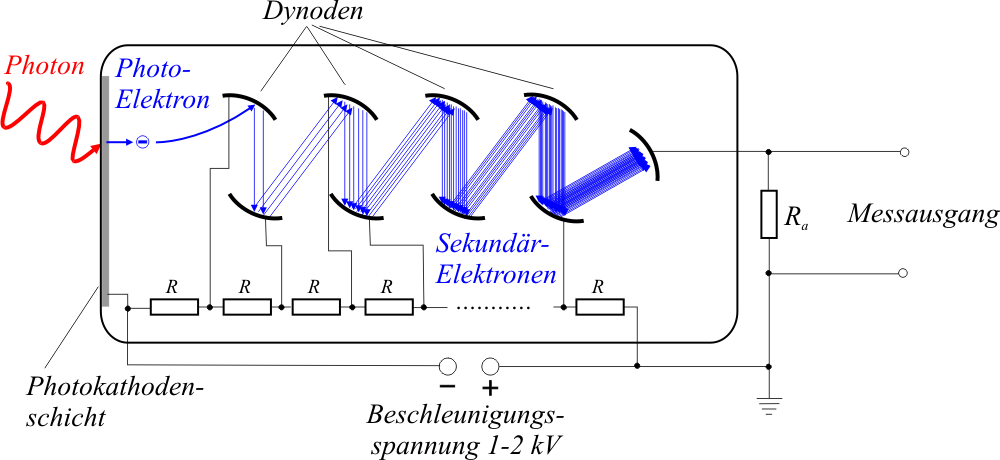
\includegraphics[width=0.85\textwidth]{images/Photomultiplier_schema_de.png}
	\caption{Schematik Photoelektronenvervielfacher \cite{Bild_Photomultiplier}}
	\label{theorie_PEV}
\end{figure}

Dort werden durch das Szintillationsphoton Elektronen aus einer Photokathode ausgeschlagen, durch angelegte Spannung zur ersten Dynode beschleunigt wo sie mit der gewonnenen kinetischen Energie weitere Elektronen auschlagen. Dieser Prozess wird einige male wiederholt bis ein messbarer elektrischer Impuls an der Anode entstehen kann.

\subsubsection{Compton-Streuung}

Die Compton-Streuung beschreibt das elastische Streuen eines Photons an einem (quasi-)freien Elektron. Dabei wird ein Teil der Energie des einfallenden Photons auf das Elektron übertragen, was zu einer Änderung der Wellenlänge des Photons führt.

\begin{figure}[ht]
	\centering
    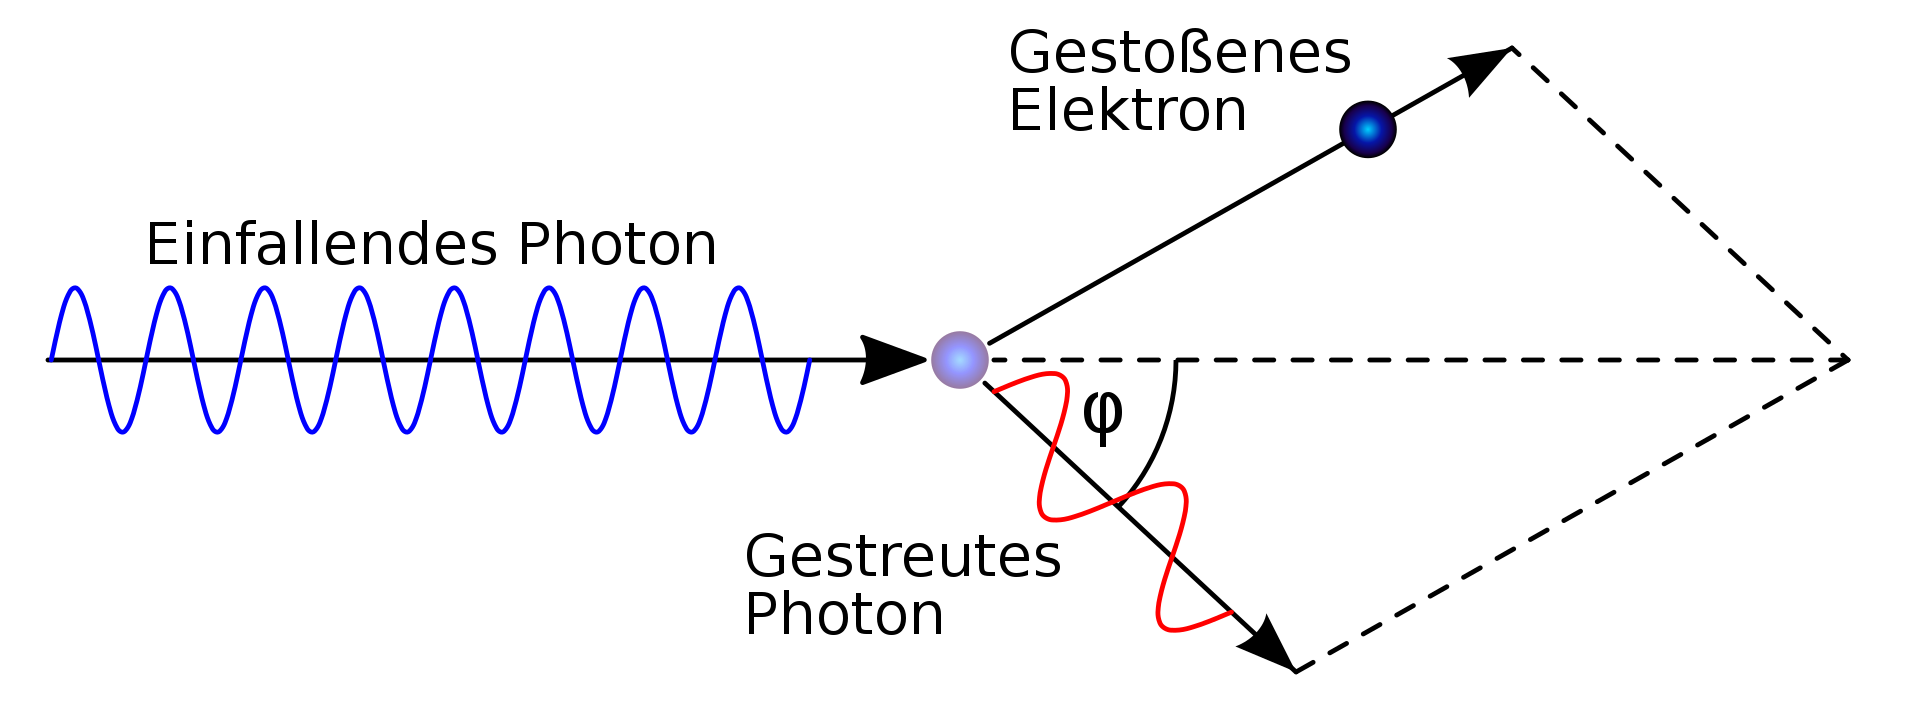
\includegraphics[width=0.85\textwidth]{images/The-geometry-of-Compton-scattering-showing-the-directions-of-the-scattered-photon-and.png}
	\caption{Schematik Compton-Streuung \cite{Bild_Compton_Streuung}}
	\label{theorie_Compton_Streuuung}
\end{figure}

Bei den in diesem Versuch verwendeten Photonenenergien tritt dieser Effekt in beiden Detektoren vorwiegend auf.
Die Energie des des gestreuten Photons $E'_{\gamma}(\varphi)$ in Abhängigkeit des Streuwinkels kann durch folgende Gleichung beschrieben werden:

\begin{gather}
    E'_{\gamma}(\varphi) = \frac{E_{\gamma}}{1 + \frac{E_{\gamma}}{m_{e} c^{2}} (1 - \cos (\varphi))}
\end{gather}

Dabei ist $\varphi$ der Streuungswinkel (s. Abb. \ref{theorie_Compton_Streuuung}), $E_{\gamma}$ die Energie des einfallenden Photons, $m_{e}$ die Masse eines Elektrons und $c$ die Vakuumlichtgeschwindigkeit.

\subsection{Vollenergiepeakanalyse}

Wie bereits erwähnt wird die Vollenergiepeakanalyse verwendet um den HPGe-Detektor zu kalibrieren. Das Ziel ist einen Zusammenhang zwischen den Kanälen des analog-to-digital-converters des HPGe-Detektors und den entsprechenden detektierten Photonenenergien zu finden (Also eine Funktion $E(\text{Kanal } i)$). Da Germanium bei den verwendeten Photonenenergien auch dem inneren Photoeffekt unterliegt bei dem die gesamte Energie des Photons im Detektor deponiert wird, finden sich im aufgenommenen Spektrum auffällige, hohe Peaks. Da wir die Energien der ausgesendeten Photonen der verwendeten Strahlenquellen kennen können wir diese Energien eben jenen Kanälen zuordnen bei denen die Peaks im Spektrum auftreten. Für die restlichen Kanäle wird dieser Zusammenhang dann extrapoliert (z.B. linearer oder quadratischer Fit) und man hat damit den Detektor kalibriert.

\subsection{Weitwinkel-Compton-Koinzidenz-Methode}

Die WCKM wird verwendet um den Szintillator zu kalibrieren. Aufgrund der niedrigen effektiven Kernladungszahl des organischen Szintillatormaterials findet man keine Vollenergiepeaks im Spektrum, jedoch findet die Compton-Streuung bei den verwendeten Photonenenergien vermehrt statt. Die Idee ist nun nur einen Teil der Energie der einfallenden Photonen über die Compton-Streuung im Szintillator zu deponieren, und die restliche Energie des Photons mittels eines anderen Detektors (bei uns der HPGe-Detektor) zu erfassen. Da wir die ursprüngliche Energie des Photons aus den Strahlungsquellen kennen und die Restenergie im zweiten Detektor erfasst wurde können wir die im Szintillator deponierte Energie bestimmen:

\begin{gather}
    E_{\text{Szintillator}} = E_{\text{Photon}} - E_{\text{sekundärer Detektor}}
    \label{theorie_Koinz}
\end{gather}

Wobei $E_{\text{Szintillator}}$ die im Szintillator deponierte Energie ist, $E_{\text{Photon}}$ die Energie des Photons vor der Streuung am Szintillator ist und $E_{\text{sekundärer Detektor}}$ die im sekundären Detektor deponierte Energie ist.

Eine wichtiger Aspekt dieser Kalibrierung wurde bis hierhin noch unterschlagen, denn es stellt sich noch die Frage woher man weiß das ein Photon erst im Szintillator gestreut und dann im sekundären Detektor absorbiert wurde. Hierbei hilft uns das Konzept der Koinzidenz: wird ein Signal im Szintillationsdetektor erfasst wartet man eine bestimmte Zeit ab und schaut währenddessen ob im sekundären Detektor auch ein Signal erfasst wird. Sollte dies der Fall sein so nimmt man die entsprechenden Messwerte beider Detektoren auf, ansonsten lässt man die Messung fallen. Die Idee ist hierbei natürlich möglichst Ereignisse herauszufiltern bei denen das Photon vom Szintillator in die Richtung des sekundären Detektors gestreut und in jenem dann auch absorbiert wurden. Aber das der beschriebene Vorgang nicht außschließlich solche Ereignisse herausfiltert ist auch sofort klar, so kann zum Beispiel nachdem das Photon im Szintillator registriert wurde aber nicht in Richtung des sekundären Detektors fliegt ein anderes Teilchen (z.B. ebenfalls von der Strahlungsquelle) zufällig im sekundären Detektor registriert werden. Man spricht bei solchen Ereignissen von zufälligen Koinzidenzen. Es gilt sicherzustellen das die zufälligen Koinzidenzen die gewollten nicht maßgebich übersteigen, da sonst die gewollten Koinzidenzen nicht mehr von den zufälligen zu unterscheiden sind.

Mithilfe der koinzidenten Ereignisse ist die lineare Beziehung in Gleichung \ref{theorie_Koinz} in einem Histogramm abbildbar. Sie ist als diagonale Gerade erkennbar wenn man die gemessenen Kanäle der beiden Detektoren gegeneinander aufträgt. Sie wird dann durch fitting zu einer Energiekalibrierung führen.
